\documentclass[11pt]{article}
\usepackage[a4paper,margin=1in]{geometry}
\usepackage{amsmath,amssymb}
\usepackage[T1]{fontenc}
\usepackage{lmodern}
\usepackage{microtype}
\usepackage{graphicx}
\usepackage{xcolor}

\setlength{\parindent}{0pt}
\setlength{\parskip}{0.5em}

\newcommand{\promptbox}[1]{%
  \begingroup\setlength{\fboxsep}{10pt}\noindent
  \colorbox{blue!8}{\parbox{\dimexpr\linewidth-2\fboxsep\relax}{\textbf{Prompt. }#1}}
  \endgroup
}
\newcommand{\resultbox}[1]{%
  \begingroup\setlength{\fboxsep}{10pt}\noindent
  \colorbox{purple!8}{\parbox{\dimexpr\linewidth-2\fboxsep\relax}{\textbf{Result. }#1}}
  \endgroup
}
\newcommand{\examplebox}[1]{%
  \begingroup\setlength{\fboxsep}{10pt}\noindent
  \colorbox{green!8}{\parbox{\dimexpr\linewidth-2\fboxsep\relax}{\textbf{Example. }#1}}
  \endgroup
}

\title{\textbf{Book 1 --- Lecture 1 --- Interlude 1 --- Exercise 1}\\[2mm]
\large Plotting Four Introductory Functions}
\author{}
\date{}

\begin{document}
\maketitle

\promptbox{Using a graphing calculator or a program like Mathematica, plot each
of the following functions:}
\[
\begin{aligned}
f(t) &= t^4 + 3t^3 - 12t^2 + t - 6, \\
g(x) &= \sin(x) - \cos(x), \\
\theta(\alpha) &= e^\alpha + \alpha\ln(\alpha), \\
x(t) &= \sin^2(t) - \cos(t).
\end{aligned}
\]

\section*{Notes Before Plotting}
\begin{itemize}
  \item \(\theta(\alpha)\) is only defined for \(\alpha>0\), because
  \(\ln(\alpha)\) needs a positive argument.
  \item \(f(t)\) is a quartic polynomial, so it grows to \(+\infty\) for large
  positive and negative \(t\).
  \item \(g(x)\) and \(x(t)\) are bounded oscillatory functions built from
  sine/cosine terms.
\end{itemize}

\section*{Example Plotting Windows}
\begin{itemize}
  \item \(t\in[-4,4]\) for \(f(t)\)
  \item \(x\in[-2\pi,2\pi]\) for \(g(x)\)
  \item \(\alpha\in[0.05,4]\) for \(\theta(\alpha)\) (avoid \(\alpha=0\))
  \item \(t\in[-2\pi,2\pi]\) for \(x(t)\)
\end{itemize}

These are starting points; zooming in/out helps identify turning points and
global behavior.

\resultbox{A useful first pass is to use windows
\(t\in[-4,4]\), \(x\in[-2\pi,2\pi]\), and \(\alpha\in[0.05,4]\).}

\examplebox{For \(\theta(\alpha)=e^\alpha+\alpha\ln(\alpha)\), the logarithm
term enforces \(\alpha>0\), so avoid \(\alpha=0\) in plotted ranges.}

\section*{Static Plot Figure}
\begin{center}
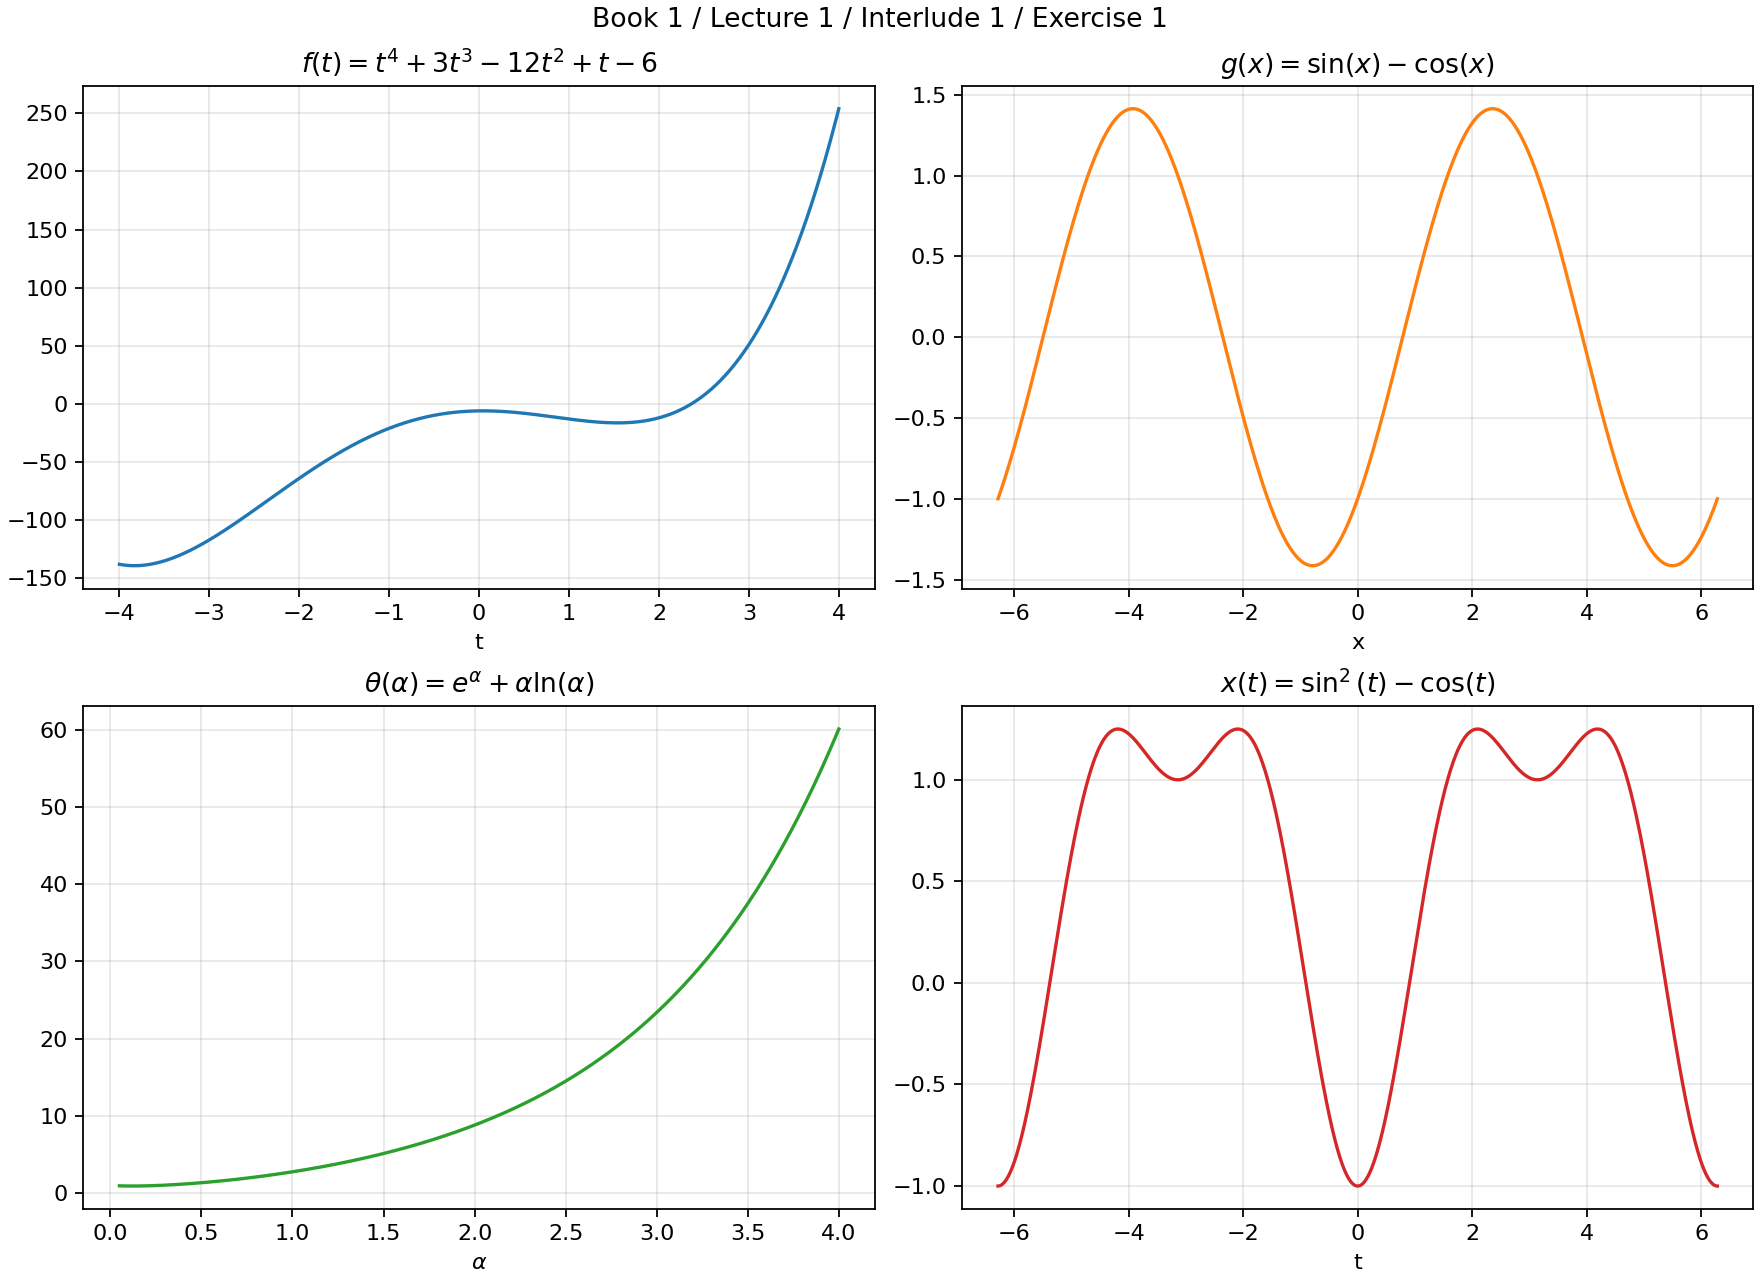
\includegraphics[width=\textwidth]{exercise-01-plots.png}
\end{center}

\end{document}
